\documentclass[12pt]{article}
\usepackage[a4paper, total={6.27in, 9.19in}]{geometry}
\usepackage[utf8]{inputenc}
\usepackage{hyperref}
\usepackage{amsmath, mathtools, amsthm}
\usepackage{thmtools}
\usepackage{amsfonts}
\usepackage{graphicx, caption, subcaption}
\usepackage{tikz}
\usepackage{fancyhdr}
\usepackage{siunitx}

%temp
\usepackage{lipsum}
%temp

\pagestyle{fancy}
\theoremstyle{definition}
\newtheorem{problem}[section]{Question}
\newtheorem{subproblem}{}[section]
\renewcommand{\thesubproblem}{(\roman{subproblem})}
\newcommand{\github}{(insert github link here)}



\newtheorem{test}[section]{Test}

\begin{document}
\def\sphoyear{20XX}
\setcounter{section}{0}
% Headers and Descriptions
\fancyhead[L]{\textbf{SPhO \sphoyear}} \fancyhead[R]{\textbf{Questions}}


\begin{titlepage}
\centering

{\Huge\bfseries SPhO \sphoyear}

\vspace{1cm}

{\LARGE Problem Set}

\vspace{2cm}

{\Large Compiled by: Tan Chien Hao, \texttt{www.tchlabs.net}}

\vspace{2cm}

{\Large Edited/Proofread by: Keith Chan, Sun Yu Chieh}
%Collaborators please feel free to add on!

\vspace{2cm}

{\large Suggest changes at: \github}


\vfill

{\itshape Last edited: \today}
\end{titlepage}


\begin{problem}
    \lipsum[2]
    \begin{subproblem}
        Hello
    \end{subproblem}
    \begin{subproblem}
        Hello
    \end{subproblem}
\end{problem}

\begin{problem}
    \lipsum[2]
    \begin{subproblem}
        Hello
    \end{subproblem}
    \begin{subproblem}
        Hello
    \end{subproblem}
\end{problem}[2]

\begin{test}[2]
Hello
\end{test}



\def\sphoyear{2010}
\setcounter{section}{0}
% Headers and Descriptions
\fancyhead[L]{\textbf{SPhO \sphoyear}} \fancyhead[R]{\textbf{Questions}}


\begin{titlepage}
\centering

{\Huge\bfseries SPhO \sphoyear}

\vspace{1cm}

{\LARGE Problem Set}

\vspace{2cm}

{\Large Compiled by: Tan Chien Hao, \texttt{www.tchlabs.net}}

\vspace{2cm}

{\Large Edited/Proofread by: Keith Chan, Sun Yu Chieh}
%Collaborators please feel free to add on!

\vspace{2cm}

{\large Suggest changes at: \github}


\vfill

{\itshape Last edited: \today}
\end{titlepage}



\begin{problem}
    In 1899, Max Planck introduced the units $\hbar=\frac{h}{2\pi}$, $c$ and $G$, where $h$ is the Planck constant, $c$ is the speed of light in vacuo and $G$ is the Newton gravitational constant so that the force between two bodies of masses $m_1$ and $m_2$ placed a distance $r$ apart is given by \[F=G\frac{m_1 m_2}{r_2}\]

    \begin{subproblem}
        In terms of these Planck units, write down the dimensions of mass, length and time. These quantities are called the Planck mass $M_{pl}$, the Planck length $l_{pl}$ and the Planck time $t_{pl}$. \hfill $[9]$
    \end{subproblem}

    \begin{subproblem}
        Find the value of $M_{pl}$ in SI (i.e. metres-kilogramme-seconds, mks) units.
    \end{subproblem}

    \begin{subproblem}
        Find the ratio \[\frac{E_{grav}}{m_e c^2}\] where $E_{grav}$ is the gravitational energy between two electrons separated by a distance equal to the Compton wavelength of an electron of mass $m_e$.
    \end{subproblem}

    \begin{subproblem}
        Consider a particle of mass $M_{pl}$. Find the ratio \[\frac{E_{grav}}{M_{pl} c^2}\] where $E_{grav}$  is the gravitational energy between two such particles separated by a distance equal to their own Compton wavelength. Thus, $M_{pl}$ can be interpreted as the mass scale that quantum gravitational effects become important. 

        
        [Note: The energy of a photon with the Compton wavelength of a particle is the same as the rest mass of the particle.]


    \end{subproblem}
\end{problem}

\begin{problem}
    A block of mass $M$ rests on a fixed plane inclined at angle $\theta$. A horizontal force of $Mg$ is applied to the block, as shown in Fig. \ref{2010q2}. The coefficient of static friction between the block and the plane is $\mu$.
    \begin{figure}[h]
        \centering
        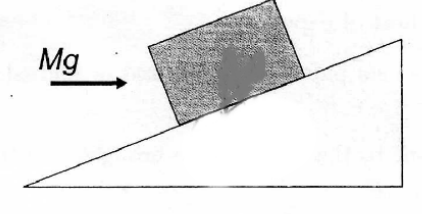
\includegraphics[width=0.5 \linewidth]{spho_book_TYS_images/2010q2.png}
        \caption{Horizontal force on a block.} \label{2010q2}
    \end{figure}
    \begin{subproblem}
        Assuming that the friction force between the block and the plane is large enough to keep the block at rest, determine the magnitude of the normal and friction forces (call them $N$ and $F_y$ ) that the plane exerts on the block in terms of $M$ and $\mu$.
    \end{subproblem}

    \begin{subproblem}
        Determine the range of angles $\theta$ for which the block remain at rest on the plane in terms of $\mu$. 
    \end{subproblem}
\end{problem}


\begin{problem}
A mobile is formed by supporting four metal butterflies of equal mass $m$ from a string of length $L$. The points of support are evenly spaced a distance $\ell$ apart as shown in Figure \ref{2010q3}. The string forms an angle $\theta_{1}$ with the ceiling at each end point. The center section of string is horizontal. 
    \begin{subproblem}
        Find the tension in each section of string in terms of $\theta_{1}, m$, and $g$.
    \end{subproblem}
    
    \begin{subproblem} 
        Find the angle $\theta_{2}$, in terms of $\theta_{1}$. 
    \end{subproblem}
    
    \begin{subproblem}
    Show that the distance $D$ between the end points of the string is
    \[D=\frac{L}{5}\left(a \cos \theta_{1}+b \cos \left[\tan ^{-1}\left(\frac{1}{2} \tan \theta_{1}\right)\right]+1\right)\]
    where $a$ and $b$ are constants to be determined. State the values of $a$ and $b$.
    \end{subproblem}

    \begin{figure}[h]
        \centering
        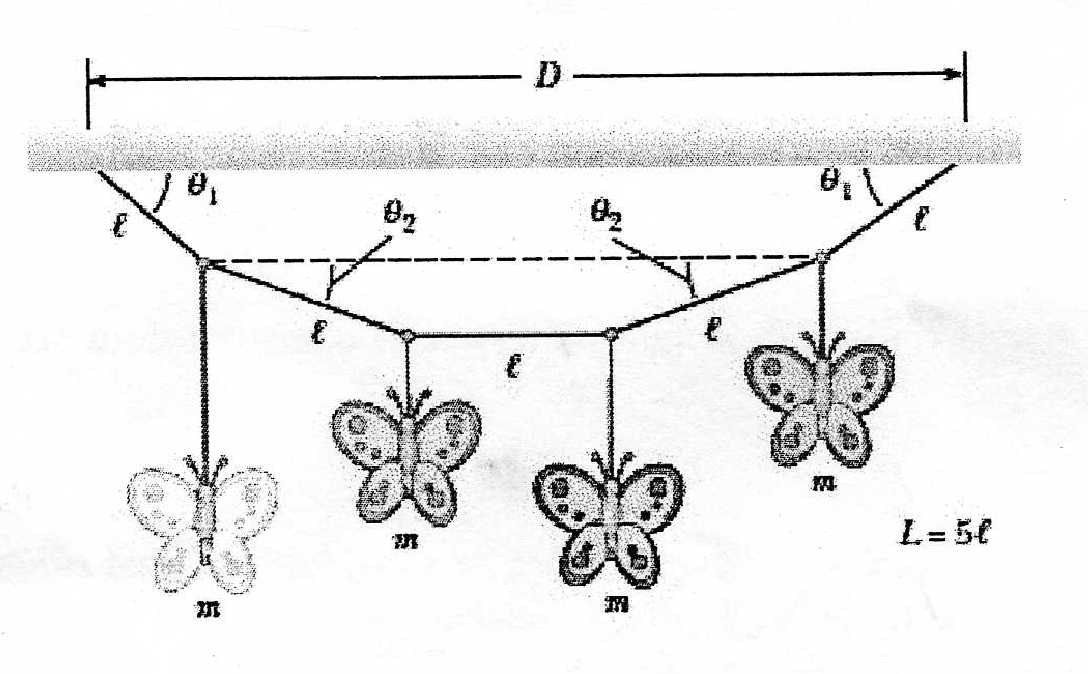
\includegraphics[width=\linewidth]{spho_book_TYS_images/2010q3.png}
        \caption{A mobile is formed by supporting four metal butterflies of equal mass $m$.} \label{2010q3}
    \end{figure}
\end{problem}

\begin{problem}
    A $\qty{670}{\kg}$ meteorite is composed of aluminium. At a distance far from the Earth, its temperature is $\qty{-15}{\degreeCelsius}$ and it moves with a speed of $\qty{14.0}{\km\per\s}$ relative to the Earth. As it crashes into the planet, the resulting additional internal energy is shared equally between the meteor and the planet. Assuming that all of the material of the meteor rises momentarily to the same final temperature, determine this temperature. You may also assume that the specific heat of liquid and of gaseous aluminium is $\qty{1170}{\J\per\kg\per\K}$, the latent heat of fusion and vaporisation of aluminium are $\qty{3.97e5}{\J\per\kg}$ and $\qty{1.14e7}{\J\per\kg}$ respectvely, and the melting point and boiling point of aluminium are $\qty{660}{\K}$ and $\qty{2450}{\K}$ respectively.
\end{problem}


\begin{problem}
    A pion at rest with a mass $m_{\pi}$ decays to a muon of mass $m_{\mu}$ and an antineutrino of negligible mass. The reaction is written as $\pi^{-} \rightarrow \mu^{-}+\bar{\nu}$. Calculate the kinetic energy of the muon and the energy of the antineutrino in electron volts. You may take $m_{\pi}=273 m_{e}$ and $m_{\mu}=207 m_{e}$ where $m_{e}$ is the rest mass of the electron.
\end{problem}

\begin{problem}
    A smaller disk of radius $r$ and mass $m$ is attached rigidly to the face of a second larger disk of radius $R$ and mass $M$ as shown in Figure \ref{2010q6}. The center of the small disk is located at the edge of the large disk. The large disk is mounted at its center on a frictionless axle. The assembly is rotated through a small angle $\theta$ from its equilibrium position and released.
    \begin{figure}[h]
	   \centering
	   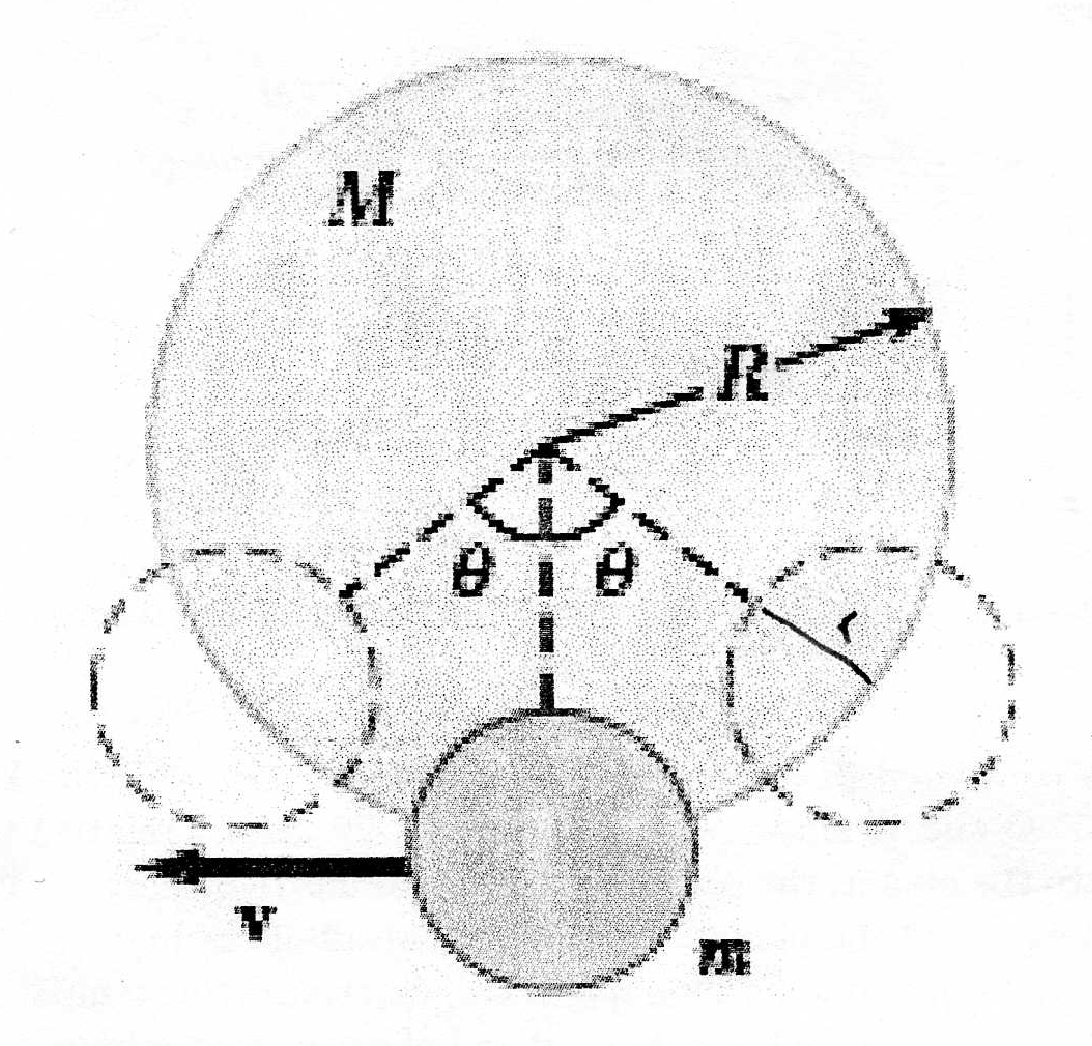
\includegraphics[width=0.5\linewidth]{spho_book_TYS_images/2010q6.png}
	   \caption{A smaller disk of radius $r$ and mass $m$ is attached rigidly to the face of a second larger disk of radius $R$ and mass $M$}\label{2010q6}
    \end{figure}
    \begin{subproblem}
        Show that the speed of the center of the small disk as it passes through the equilibrium position is
        \[v=\alpha\left[\frac{R g(1-\cos \theta)}{(M / m)+(r / R)^{2}+\beta}\right]^{1 / 2}\]
        where $\alpha$ and $\beta$ are constants to be determined. State the values of these constants.
    \end{subproblem}
    
    \begin{subproblem}
        Determine the period of the motion in terms of $M, m, R$ and $r$.
    \end{subproblem}
\end{problem}

\begin{problem}
    An electric motor turns a flywheel through a drive belt that joins a pulley on the motor and a pulley that is rigidly attached to the flywheel, as shown in Figure \ref{2010q7}. The flywheel is a solid disk with a mass of $\qty{80.0}{\kg}$ and a diameter of $\qty{1.25}{\m}$. It turns on a frictionless axle. Its pulley has a much smaller mass and a radius of $\qty{0.230}{\m}$. If the tension in the upper (taut) segment of the belt is $\qty{135}{\N}$ and the flywheel has a clockwise angular acceleration of $\qty{1.67}{\radian\per\s\squared}$, find the tension in the lower (slack) segment of the belt.
    \begin{figure}[h]
	    \centering
	    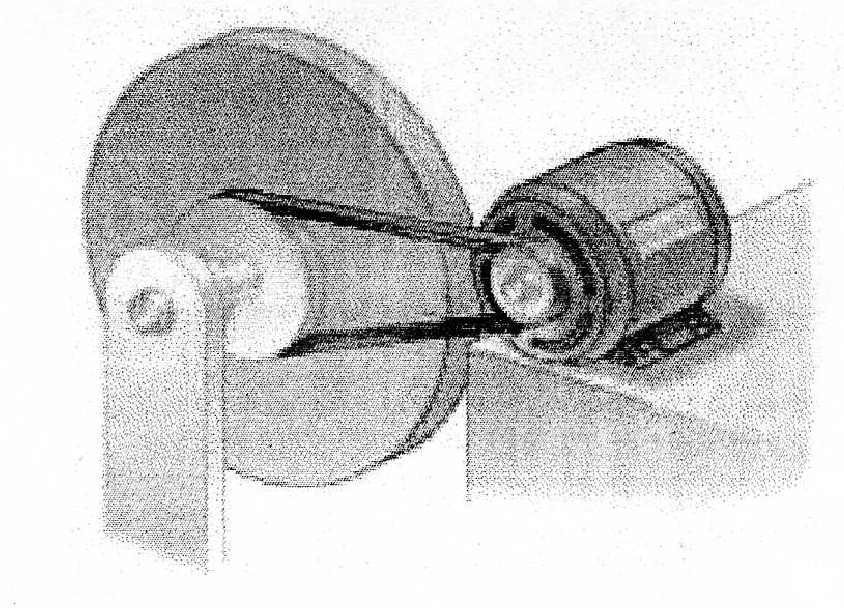
\includegraphics[width=0.5\linewidth]{spho_book_TYS_images/2010q7.png}
	    \caption{An electric motor turns a flywheel through a drive belt that joins a pulley on}\label{2010q7}
    \end{figure}
\end{problem}

\begin{problem}
    A plano-concave lens having index of refraction $1.50$ is placed on a flat glass plate, as shown in Figure \ref{2010q8}. Its curved surface, with radius of curvature $\qty{8.00}{\m}$, is on the bottom. The lens is illuminated from above with yellow sodium light of wavelength $\qty{589}{\nm}$, and a series of concentric bright and dark rings is observed by reflection. The interference pattern has a dark spot at the centre, surrounded by 50 dark rings, of which the largest is at the outer edge of the lens.
    \begin{figure}[h]
	    \centering
	    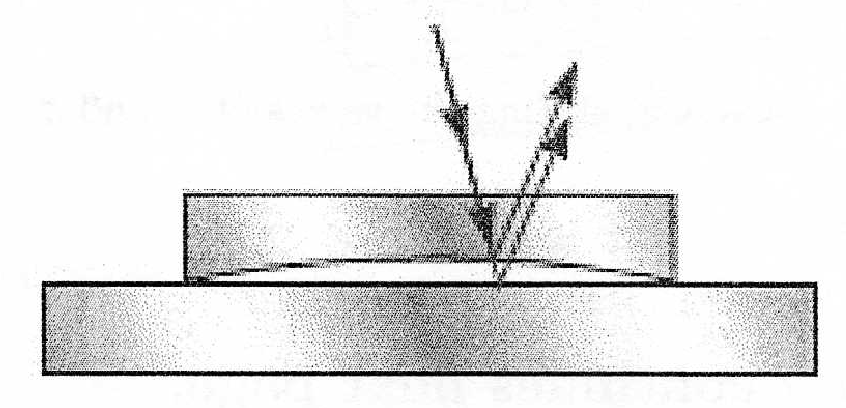
\includegraphics[width=0.5\linewidth]{spho_book_TYS_images/2010q8.png}
	    \caption{A plano-concave lens placed on a flat glass plate} \label{2010q8}
    \end{figure}
    \begin{subproblem}
        What is the thickness of the air layer at the centre of the interference pattern?
    \end{subproblem}
    \begin{subproblem}
        Calculate the radius of the outermost dark ring.
    \end{subproblem}
    \begin{subproblem}
        Find the focal length of the lens.
    \end{subproblem}
\end{problem}

\begin{problem}
    \begin{partproblem}
        A toroid has a major radius $R$ and a minor radius $r$ and it is tightly wound with $N$ turns of wire, as shown in Figure \ref{2010q9}. If $R>>r$, the magnetic field in the region enclosed by the wire of the torus, of cross-sectional area $A=\pi r^{2}$, is essentially the same as the magnetic field of a solenoid that has been bent into a large circle of radius $R$.\\
        \begin{figure}[h]
	        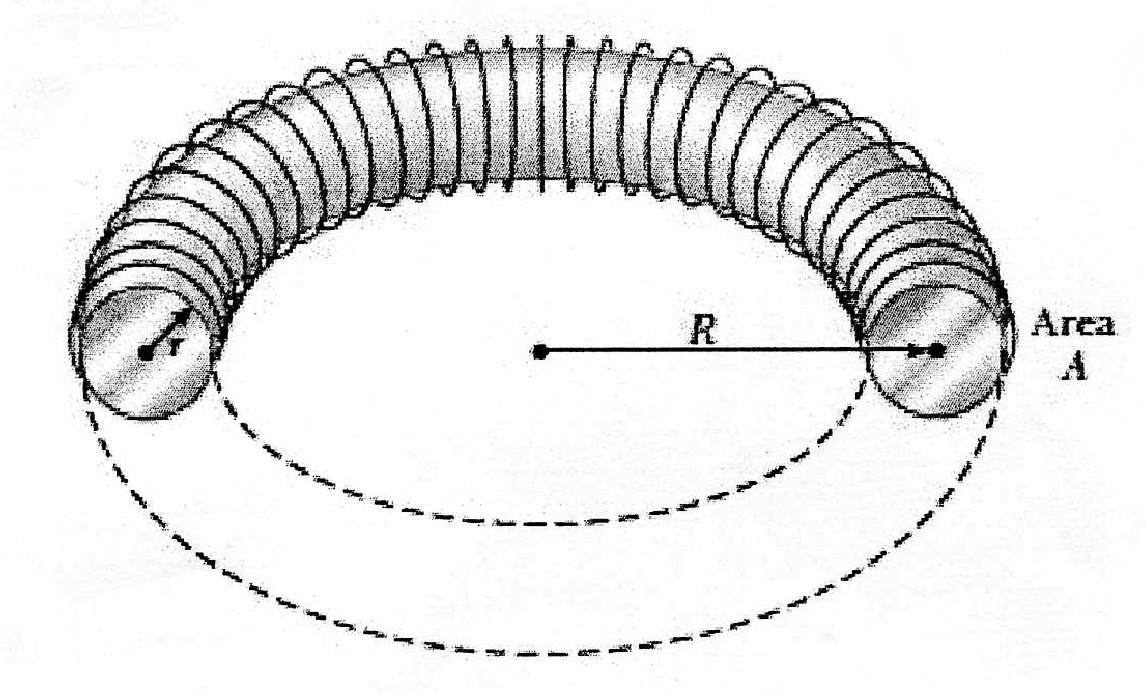
\includegraphics[width=0.8\linewidth]{spho_book_TYS_images/2010q9.png}
	        \caption{A toroid has a major radius $R$ and a minor radius $r$ and it is tightly wound with $N$ turns of wire.} \label{2010q9}
        \end{figure}
        Show that the self-inductance of such a toroid is approximately
        \[L \approx \kappa \mu_{0} \frac{N^{\alpha} A}{R}\]
        where $\kappa$ and $\alpha$ are constants. State the values of $\kappa$ and $\alpha$.
    \end{partproblem}

    \begin{partproblem}
        The toroid in Figure \ref{2010q9} with $N$ turns of wire is now replaced by one with a rectangular cross section. Its inner and outer radii are $a$ and $b$, respectively. The cross-section is a rectangle of length $b-a$ and breadth $h$.
        \begin{figure}[h]
	          \centering
	        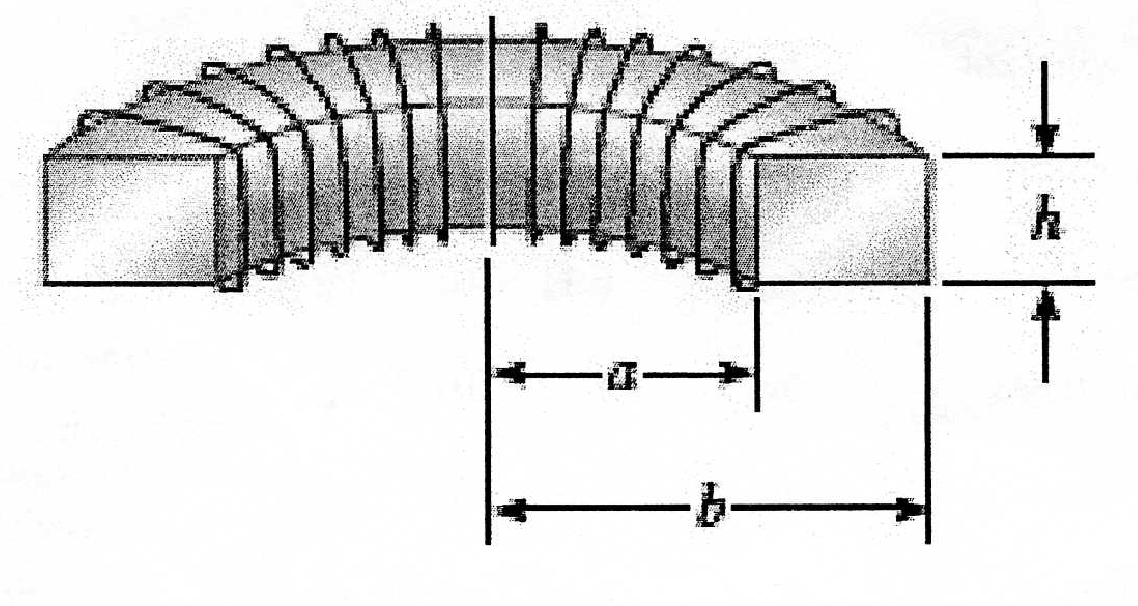
\includegraphics[width=0.8\linewidth]{spho_book_TYS_images/2010q9_2.png}
	        \caption{A toroid with a rectangular cross-section.} \label{2010q9_2}
        \end{figure}
        \begin{subproblem}
            Show that the inductance of the toroid is
            \[L=\kappa^{\prime} \mu_{0} \frac{N^{\beta} h}{R} \ln \frac{b}{a}\]
            where $\kappa^{\prime}$ and $\beta$ are constants, stating the values of $\kappa^{\prime}$ and $\beta$.
        \end{subproblem}

        \begin{subproblem}
            Compute the self-inductance of a 500-turn toroid for which $a=\qty{10.0}{\cm}$, $b=\qty{12.0}{\cm}$, and $\qty{1.00}{\cm}$. In part (a), an approximate expression for the inductances of a toroid with $R>>r$ was derived. If the calculations in part (b) (ii) were done using this approximate expression for self-inductance, what is the percentage error in the result?
        \end{subproblem}
    \end{partproblem}
\end{problem}

\begin{problem}
    An empty box of total mass $M$ with perfectly reflecting walls is at rest in the lab frame. Then electromagnetic standing waves are introduced along the $x$ direction, consisting of $N$ photons, each of frequency $\nu$ as shown in Fig. 8. Determine the rest mass of the system (box + photons) when the photons are present.
    \begin{figure}[h]
	    \centering
	    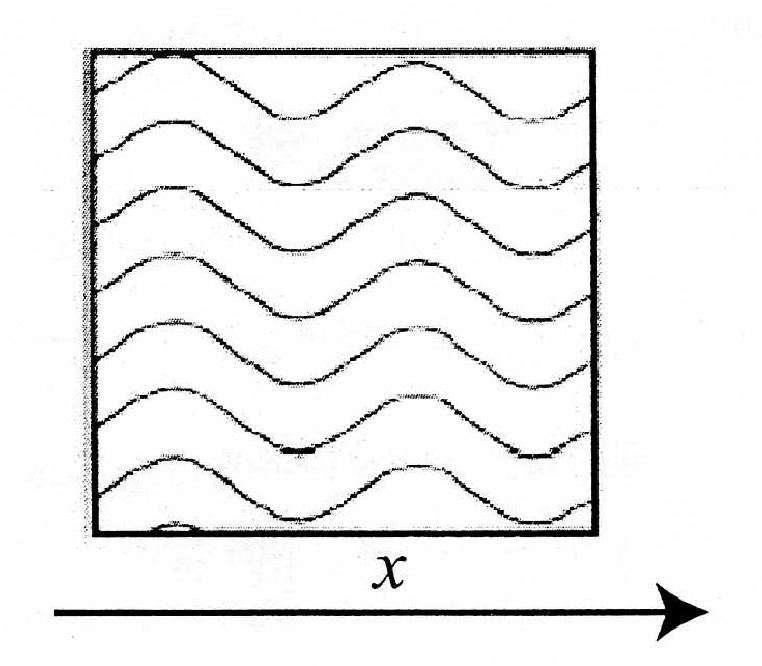
\includegraphics[width=0.5\linewidth]{spho_book_TYS_images/2010q10.png}
	    \caption{An empty box of total mass $M$ with perfectly reflecting walls is at rest in the lab frame.}
    \end{figure}
\end{problem}
\def\sphoyear{2011}
\setcounter{section}{0}
% Headers and Descriptions
\fancyhead[L]{\textbf{SPhO \sphoyear}} \fancyhead[R]{\textbf{Questions}}


\begin{titlepage}
\centering

{\Huge\bfseries SPhO \sphoyear}

\vspace{1cm}

{\LARGE Problem Set}

\vspace{2cm}

{\Large Compiled by: Tan Chien Hao, \texttt{www.tchlabs.net}}

\vspace{2cm}

{\Large Edited/Proofread by: Keith Chan, Sun Yu Chieh}
%Collaborators please feel free to add on!

\vspace{2cm}

{\large Suggest changes at: \github}


\vfill

{\itshape Last edited: \today}
\end{titlepage}

\begin{problem}
    A pendulum consists of a copper sphere of radius $R$ and density $\varrho$ suspended from a string. Due to the drag from the air the amplitude of the oscillation $A$ decays with time $t$ as
    \[A=A_0 \exp(-\gamma t)\]
    where $\gamma=\frac{9 \eta}{4 R^{2} \varrho}$. $A_0$ is the initial amplitude of the pendulum and $\eta$ is the viscosity of air. The measurement of the amplitudes is accurate to $1\%$ with other measurements provided below
    \sisetup{uncertainty-mode = separate}
    \begin{align*}
        &\eta=\qty{1.78\pm 0.02e-5}{\kg\per\m\per\s}\\
	    &R=\qty{5.2\pm 0.2}{\mm} \\
	    &\varrho=\qty{0.89\pm 0.05e3}{\kg\per\m\cubed}
    \end{align*}
    Evaluate the time taken for the amplitude to fall to $85\%$ of the initial amplitude $A_{0}$ and the error in this quantity. State the parameter that contributes the biggest error to the final result.
\hfill{[8]}\end{problem}

\begin{problem}
    In this question you are asked to make reasoned estimates and assumptions. These must be clearly stated.
    \begin{subproblem}
        Figure \ref{2011q2} shows an equilateral glass prism illuminated by a 100 W laser beam of wavelength $\lambda=\qty{600}{\nm}$. The refractive index of the glass of the prism is $1.50$ at $\lambda=600 \mathrm{~nm}$. The path of the light in the prism is parallel to the base of the prism. Calculate the change in weight of the prism when the beam is switched on.
        \begin{figure}[h]
	        \centering
	        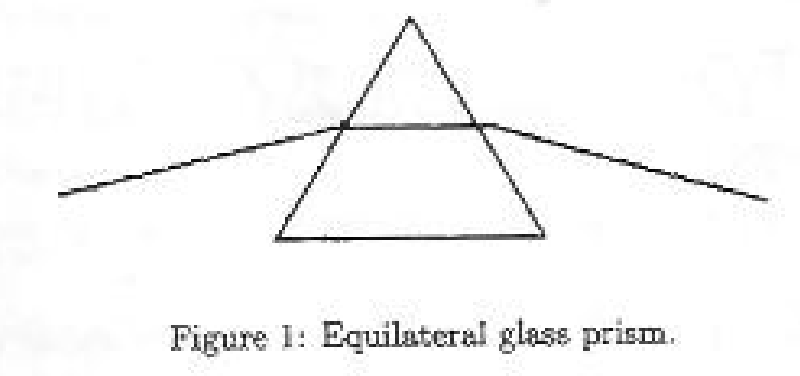
\includegraphics[width=0.8\linewidth]{spho_book_TYS_images/2011q2.png}
	        \caption{Equilateral glass prism} \label{2011q2}
        \end{figure}
    \hfill{[4]}\end{subproblem}
    
    \begin{subproblem}
        Optical tweezers, which are composed of two lasers beams, are able to manipulate small transparent spheres. Explain clearly how this can be done and why at least two beams are needed.
    \hfill{[3]}\end{subproblem}
    
    \begin{subproblem}
        Small smoke particles in air are seen under a low magnification microscope to move randomly at speed of $0.10 \mathrm{~mm}^{-1}$. The speed of sound in air is $20 \mathrm{~m} \mathrm{~s}^{-1}$. Estimate the mass of the smoke particles.
    \hfill{[3]}\end{subproblem}
\end{problem}

\begin{problem}
    Suppose that we have a string of equally spaced beads of mass m such that their surfaces are separated by a distance $d$. The beads are free to slide without friction on 4 thin wires. Suppose that there is a constant force $F$ acting on the first bead, initially at rest, and causing it to accelerate along the wire as shown in Figure \ref{2011q3}. This force acts only on the first bead and might be created by a well directed, steady stream of air. The first bead will collide with the second, which will in turn collide with the third, and so on. Suppose that all collisions are elastic.
    \begin{figure}[h]
	    \centering
	    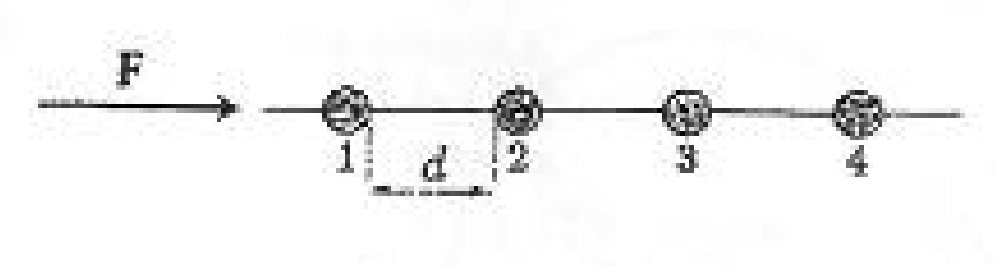
\includegraphics[width=0.7\linewidth]{spho_book_TYS_images/2011q3.png}
	    \caption{Beads on wire} \label{2011q3}
    \end{figure}
    \begin{subproblem}
        What is the speed of the first bead immediately before and immediately after its collision with the second bead?
    \hfill{[2]}\end{subproblem}

    \begin{subproblem}
        What is the speed of the second bead immediately before and immediately after its collision with the third bead?
    \hfill{[2]}\end{subproblem}

    \begin{subproblem}
        Note that the constant force is always acting upon the first bead. What is the time interval between subsequent collisions between the first and second beads? What then is the average speed of the first bead? What is the speed of the “shock wave" that travels down the wire?
    \hfill{[3]}\end{subproblem}

    \begin{subproblem}
        If the whole process is repeated, but with collisions which are perfectly inelastic, what is the terminal speed of the shock wave formed?
    \hfill{[3]}\end{subproblem}
\end{problem}

\begin{problem}
    A zoom lens system is a combination of lenses that produces a variable magnification while maintaining fixed object and image positions. The magnification is varied by moving one or more lenses along the axis. While multiple lenses are used in practice to obtain high-quality images, the effect of zooming in on an object can be demonstrated with a simple two-lens system. An object, two converging lenses, and a screen are mounted on an optical bench. The first lens, which is to the right of the object, has a focal length of $\qty{5.0}{\cm}$, and the second lens, which is to the right of the first lens, has a focal length of $\qty{10.0}{\cm}$. The screen is to the right of the second lens. Initially, an object is situated at a distance of $\qty{7.50}{\cm}$ to the left of the first lens, and the image formed on the screen has a magnification of $1.00$.
    \begin{subproblem}
        Determine the distance between the object and the screen.
    \hfill{[4]}\end{subproblem}

    \begin{subproblem}
        Both lenses are now moved along their common axis, while the object and the screen maintain fixed positions, until the image formed on the screen has - magnification of $+3.00$. Find the displacement of each lens from its initial position in (i).
    \hfill{[4]}\end{subproblem}

    \begin{subproblem}
        Can the lenses be displaced in more than one way?
    \hfill{[4]}\end{subproblem}
\end{problem}

\begin{problem}
    \begin{subproblem}
        A stick of mass density per unit length $\rho$ rests on a circle of radius $R$ (see Figure \textit{insert here}). The stick makes an angle $\theta$ with the horizontal and is tangent to the circle at its upper end. Friction exists at all points of contact, and assume that it is large enough to keep the system at rest. Find the friction force between the ground and the circle.
    \hfill{[6]}\end{subproblem}

    \begin{subproblem}
        A large number of sticks (with mass density per unit length $\rho$) and circles (with radius $R$) lean on each other, an shown in Figure \ref{2011q5}. Each stick makes an angle $\theta$ with the horizontal and is tangent to a circle at its upper end. The sticks are hinged to the ground, and every other surface is frictionless unlike in the first part of this question in (i)]. In the limit of a very large number of sticks and circles, what is the normal force between a stick and the circle it rests on very far to the right? (Assume that the last circle leans against a wall, to keep it from moving)
        \begin{figure}[h]
	        \centering
	        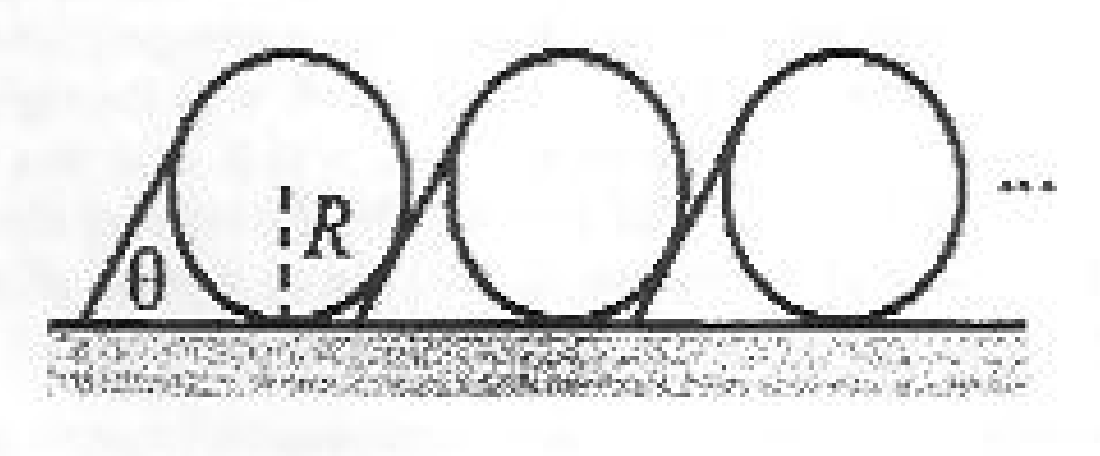
\includegraphics[width=0.7\linewidth]{spho_book_TYS_images/2011q5.png}
	        \caption{Sticks on circles}\label{2011q5}
        \end{figure}
    \hfill{[6]}\end{subproblem}
\end{problem}

\begin{problem}
    An aluminium rod $\qty{0.500}{\m}$ in length and with a cross-sectional area of $\qty{2.50}{\square\cm}$ is inserted into a thermally insulated vessel containing liquid helium at $\qty{4.20}{\K}$. The rod is initially at $\qty{300}{\K}$.
    \begin{subproblem}
        If half of the rod is inserted into the helium, how many litres of helium boil off by the time the inserted half cools to $4.20 \mathrm{~K} ?$ (Assume the upper half does not yet cool.)
    \hfill{[4]}\end{subproblem}
    \begin{subproblem}
        If the upper end of the rod is maintained at $\qty{300}{\K}$, what is the approximate boil-off rate of liquid helium after the lower half has reached $\qty{4.20}{\K}$? (Aluminium has thermal conductivity of $\qty{31.0}{\J\per\s\per\cm\per\K}$ at $\qty{4.20}{\K}$ You may ignore its temperature variation. Note that aluminium has a specific heat capacity of $\qty{902}{\J\per\kg\per\K}$ and density of $\qty{2700}{\kg\per\cubic\m}$. The density of liquid helium is $\qty{125}{\kg\per\cubic\m}$.)
    \hfill{[4]}\end{subproblem}
\end{problem}

\begin{problem}
    A soap film $(n=1.33)$ is contained within a rectangular wire frame. The frame is held vertically so that the film drains downward and forms a wedge with flat faces. The thickness of the film at the top is essentially zero. The film is viewed in reflected white light with near-normal incidence, and the first violet (the wavelength is $\qty{420}{\nm}$) interference band is observed $\qty{3.00}{\cm}$ from the top edge of the film.
    \begin{subproblem}
        Locate the first red $(\lambda=\qty{600}{\nm})$ interference band.
    \hfill{[4]}\end{subproblem}
    \begin{subproblem}
        Determine the film thickness at the positions of the violet and red bands.
    \hfill{[3]}\end{subproblem}
    \begin{subproblem}
        What is the wedge angle of the film?
    \hfill{[3]}\end{subproblem}
\end{problem}

\begin{problem}
    A solenoid of length $2 \ell$ has an inner radius $R_{1}$ and an outer radius $R_{2}$. The current through the solenoid is $I$.
    \begin{subproblem}
        Show that the magnetic flux density, $B$ at the centre of the solenoid is
        \[B=\kappa n I \ell \frac{\alpha+\left(\alpha^{2}+\beta^{2}\right)^{1 / 2}}{1+\left(1+\beta^{2}\right)^{1 / 2}}\]
        where $n$ is the number of turns per square meter and $\alpha$ and $\beta$ are functions of $R_{1}, R_{2}$ and $L$. Write down the expression for $\alpha$ and $\beta$. State the value of $\kappa$.
    \end{subproblem}
    \begin{subproblem}
        Show that the length of the wire is
        \[\ell=n V=2 \pi n\left(\alpha^{m_{1}}-1\right) \beta^{m_{1}} R_{1}^{m_{2}}\]
        where $V$ is the volume of the winding and $m_{1}, m_{2}$ and $m_{3}$ are exponents that need to be determined. State the value of $m_{1}, m_{2}$ and $m_{3}$.
    \end{subproblem}
    \begin{subproblem}
        Show that the $B$ field at the centre of the solenoid can be written as
        \[B=G\left(\frac{P \lambda \sigma}{R_{1}}\right)^{1/2}\]
        where $G$ depends on the geometry, $P$ is the dissipated power, $\lambda=\pi \pi r^{2}$ is the filling factor or fraction of the coil cross sechon oocupied by the conductor, $r$ is the radius of the wire and $\sigma$ is the conductivity.
    \hfill{[4]}\end{subproblem}
\end{problem}

\begin{problem}
    \begin{subproblem}
        A large block, with a second block sitting on top, is connected to a spring and executes horizontal simple harmonic motion as it slides across a frictionless surface with an angular frequency $\omega$. The coefficient of static friction between the two blocks is $\mu_{s}$. Derive a formula for the maximum amplitude of oscillation that the system can have if the upper block is not to slip. (Assume that the mass of the spring is negligible.)
    \hfill{[6]}\end{subproblem}
    \begin{subproblem}
        A pencil of length $L_{1}$ with the pencil point at one end and an eraser at the other end, is initially standing vertically on a table with the pencil point on the table. The pencil is let go and falls over. Derive a formula for the speed with which the eraser strikes the table, assuming that the pencil point does not move.
    \hfill{[4]}\end{subproblem}
\end{problem}


\begin{problem}
    \begin{subproblem}
        The Oscillation Project with Emulsion-tRacking Apparatus (OPERA), an experiment designed to test neutrino oscillations and exploiting the high energy muon neutrino produced at CERN Super Proton Synchrotron in Geneva and pointing towards Gran Sasso in Italy, reported that the time of flight measurements indicated that muon neutrinos travel at speed $v$ which is faster than the speed of light with $\beta=\frac{v}{c}=1+\num{1.48e-5}$, where $c$ is the speed of light in vacua. Show that it is possible for an observer moving relative to the Earth starting at CERN and moving towards Gran Sasso at some critical speed $u$ to see the muon neutrino moving backwards from Gran Sasso towards CERN and determine this critical speed.
    \end{subproblem}
    \begin{subproblem}
        A moving rod is observed to have a length of $\qty{2.00}{\m}$ and to be oriented at an angle of $\qty{30.0}{\degree}$ with respect to the direction of motion, as shown in the Figure below. The rod has a speed of $0.995\,c$.
        \begin{figure}[h]
	        \centering
	        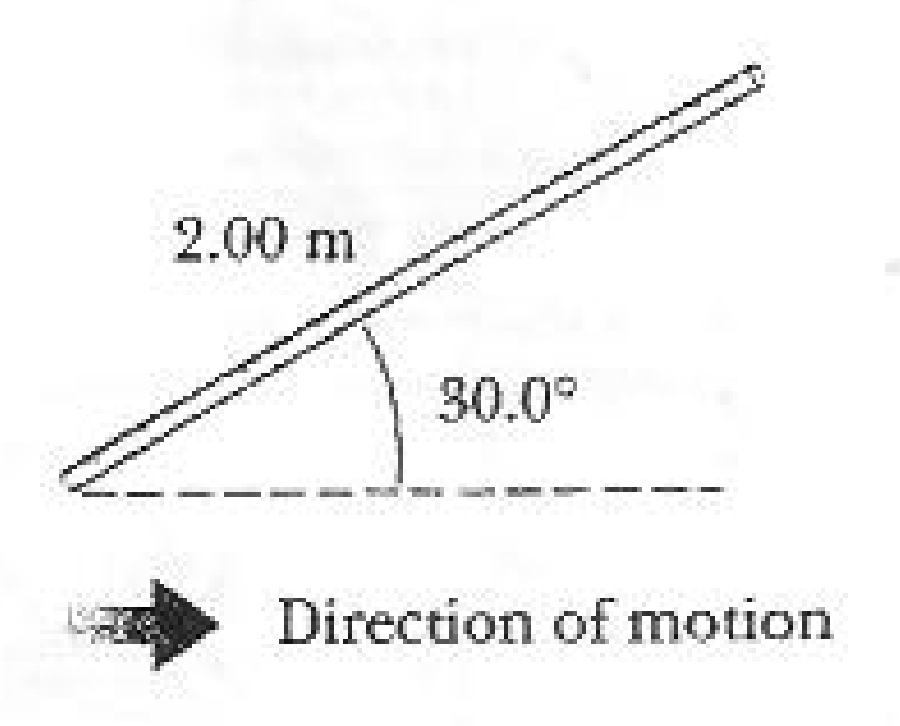
\includegraphics[width=0.7\linewidth]{spho_book_TYS_images/2011q10.png}
	          \caption{Relativistic Rod}
        \end{figure}
        \renewcommand{\theenumi}{(\alph{enumi})}
        \begin{enumerate}
            \item Determine the proper length of the rod.\hfill{[3]}
            \item What is the orientation angle in the proper frame?\hfill{[3]}
        \end{enumerate}
    \end{subproblem}
\end{problem}






\end{document}